 \documentclass[a4paper,12pt]{article} 
\usepackage[T2A]{fontenc}			
\usepackage[utf8]{inputenc}			
\usepackage[english,russian]{babel}	
\usepackage{amsmath,amsfonts,amssymb,amsthm,mathrsfs,mathtools} 
\usepackage[colorlinks, linkcolor = purple, citecolor = purple]{hyperref}
\usepackage{xcolor}
\usepackage{xpatch}
\usepackage{marvosym}
\usepackage{cancel}
\usepackage{floatrow}
\usepackage{commath}
\usepackage{upgreek}
\usepackage{lipsum}
\usepackage{mhchem}
\usepackage{chemfig}
\usepackage{multirow}
\usepackage{tikz}
\usepackage{titletoc}
\usepackage{pgfplots}
\usepackage{wrapfig}
\usepackage{chngcntr}
\usepackage{makecell}
\usepackage{stackengine,graphicx}
\usepackage{cmap}
\usepackage{indentfirst}
\usepackage{tocloft}
\usepackage{setspace}
\usepackage{titlesec}
\usepackage{soul}
\usepackage[stable]{footmisc}
\usepackage{tocloft}
\usetikzlibrary{positioning}
\usepackage{caption}
\usepackage{subfig}
\pgfplotsset{width=10cm,compat=1.9}
\tikzset{>=stealth}
\usepackage[left=2cm,right=2cm,top=2cm,bottom=3cm,bindingoffset=0cm]{geometry}
%\DeclareMathOperator*{\esssup}{ess\,sup}
\DeclareMathOperator*{\tr}{tr}
\DeclareMathOperator*{\Ker}{Ker}
\DeclareMathOperator*{\Rea}{Re}
\DeclareMathOperator*{\Ima}{Im}
\DeclareFontEncoding{LS2}{}{\noaccents@}
\DeclareFontSubstitution{LS2}{stix}{m}{n}
\DeclareSymbolFont{arrows3}{LS2}{stixtt}{m}{n}
\DeclareMathSymbol{\squareulblack}{\mathord}{arrows3}{"88}
\date{\vspace{-10pt}}
\author{Дорогинин Д.В. Б02-825бф\\
Матвеев Г.А. Б02-824бф}
\title{\textbf{Электронный парамагнитный резонанс.}}


\theoremstyle{definition}
\newtheorem*{definition}{Определение}
\newtheorem{statement}{Предложение}
\newtheorem{lemma}{Лемма}
\newtheorem{theorem}{Теорема}
\newtheorem*{theorem*}{Теорема}
\newtheorem*{corollary}{Следствие}
\newtheorem*{example}{Пример}
\setcounter{tocdepth}{2}
%\renewcommand\cftsecafterpnum{\vspace{-pt}}
%\renewcommand\cftsecafterpnum{\vspace{1pt}}
\newcommand*{\eqdef}{\mathop{\overset{\mathrm{def}}{\resizebox{\widthof{\ensuremath{\mathop{\overset{\mathrm{def}}{=}}}}}{\heightof{=}}{=}}}}
\renewcommand\qedsymbol{$\squareulblack$}
\renewcommand{\cftsecleader}{\cftdotfill{\cftdotsep}}
\newfloatcommand{capbtabbox}{table}[][\FBwidth]
\newcommand{\HH}{\mathcal{H}}
\newcommand{\DD}{\mathcal{D}}
\newcommand{\LL}{\mathcal{L}}
\newcommand{\AAA}{\mathscr{A}}
\newcommand{\SpA}{\mathcal{A}}
\newcommand{\EE}{\mathcal{E}}
\newcommand{\suml}{\sum\limits_{n=1}^\infty}
\newcommand{\sumlN}{\sum\limits_{n=1}^N}
\newcommand{\sumo}{\sum\limits_{n=0}^\infty}
\newcommand{\sumoN}{\sum\limits_{n=0}^N}
\renewcommand\cftsecfont{\normalsize}
\renewcommand\cftsubsecfont{\normalsize}
\titleformat{\section}
  {\normalfont\fontsize{16}{16}\bfseries}{\thesection}{1em}{}
\def\rlwd{.5pt}
\def\crossy{\kern.5pt\def\stacktype{L}%
 \stackon[0.65ex]{%
  \stackon[1.4ex]{%
    \stackon[1.1ex]{\rule{\rlwd}{1.8ex}}{\rule{1.4ex}{\rlwd}}%
  }{\rule{0.8ex}{\rlwd}}%
 }{\rotatebox{-20}{\rule{0.8ex}{\rlwd}}}%
\kern1pt}



\newcommand{\angstrom}{\mbox{\normalfont\AA}}


\begin{document}
\begin{titlepage}
	\begin{center}
		\large 	Московский физико-технический институт \\
		(национальный исследовательский университет) \\
		Факультет общей и прикладной физики \\
		\vspace{0.2cm}
		
		\vspace{4.5cm}
		Лабораторная работа №6.11.3  \\ \vspace{0.2cm}
		\large (Основы современной физики) \\ \vspace{0.2cm}
		\LARGE \textbf{ Измерение контактной разности потенциалов в полупроводниках }
	\end{center}
	\vspace{2.3cm} \large
	
	\begin{center}
		Работу выполнил: \\
		Дорогинин Демид,
		группа Б02-825
		\vspace{10mm}			
	\end{center}
		
	\begin{center} \vspace{60mm}
		г. Долгопрудный \\
		2021 год
	\end{center}
\end{titlepage}


\stepcounter{page}
\section*{Аннотация}
В работе определяется контактная разность потенциалов ($p$-$n$)-перехода в полупроводниковом диоде по результатам измерений температурной зависимости его сопротивления.
\section*{Теория}
Полупроводник, в который введены доноры -- атомы элементов пятой группы, создающие дополнительные <<локальные уровни>> (Рис. 1а), называются проводниками $n$-типа. В них основными носителями заряда являются электроны. Если в полупроводник введены акцепторные примеси, то есть атомы третьей группы, которые создают вблизи верхнего края волентной зоны локальные уровни, оказывающиеся пустыми при низких температурах ((Рис. 1б), то они называются полупроводниками $p$-типа. В них основными носителями заряда являются дырки.
\begin{figure}[h]
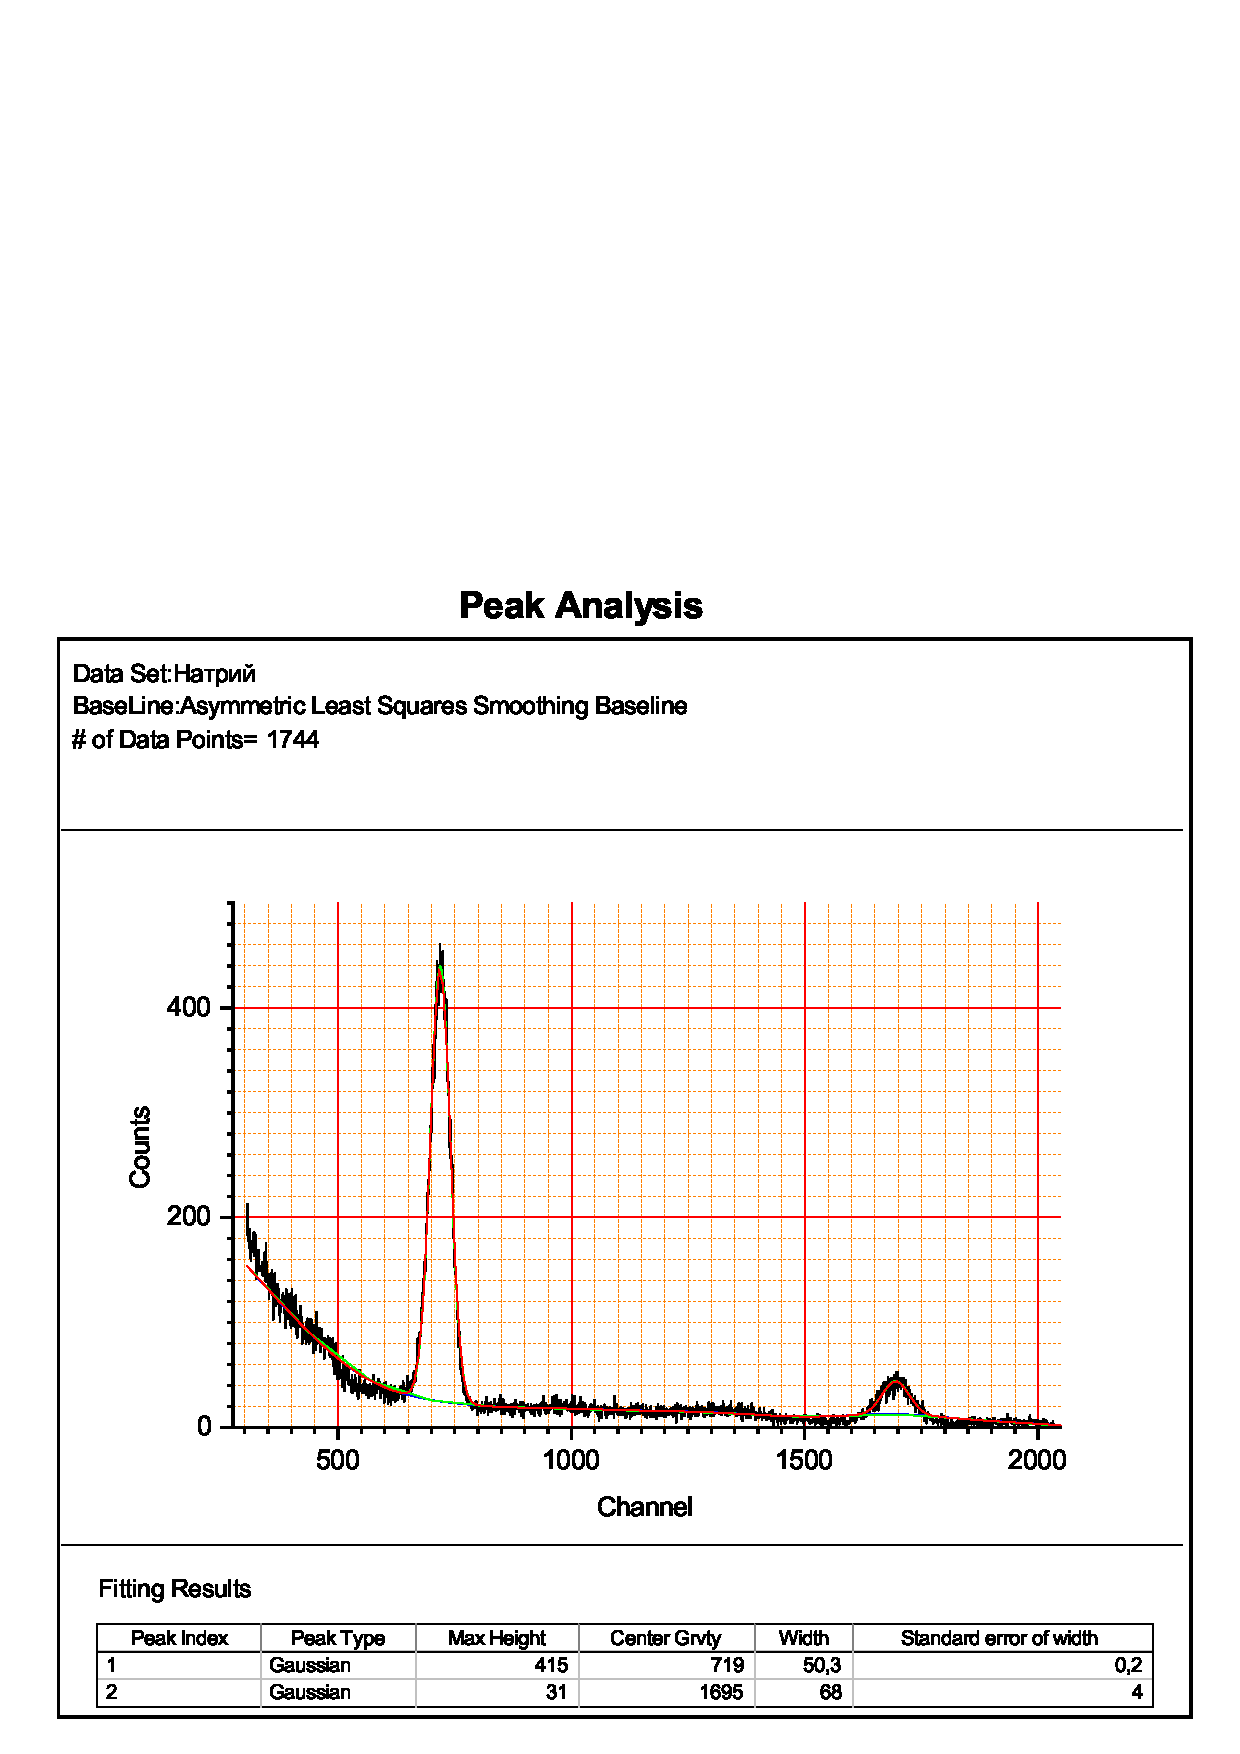
\includegraphics[width = 0.8\textwidth]{1.png}
\centering
\caption{Энергетическая схема полупроводника (а) $n$-типа; (б) $p$-типа; (в) ($p$--$n$)-типа.}
\end{figure}\\
Если привести полупроводники двух типов в соприкосновение, то произойдёт встречная диффузия основных носимтелей тока. В $n$-области вблизи перехода положительные ионы донорной примеси, заряд которых не компенсируется электронами, образуют положительных пространственный заряд. В $p$-области соответственно образуется отрицательный пространственный заряд. Таким образом, в области перехода образуется слой, обеднённый носителями тока, и сответственно возникается \textit{контактная разность потенциалов} $\Delta V$ -- потенциальный барьер, препятствующий дальнейшей диффузии основных носителей. Равновесие наступает при такой высоте потенциального барьера, что когда положения уровней Ферми в обеих областях совпадают (Рис. 1в).\\
Из-за наличия барера в условиях равновесия между концентрациями основных и неосновных носителей в $n$- и $p$- областях устанавлвается соотношение 
\[\dfrac{n_n(n-\text{область})}{n_n(p-\text{область})} = \dfrac{n_p(p-\text{область})}{n_p(n-\text{область})} = \exp\left( \dfrac{e\Delta V}{k_\text{Б}T}\right).\]
Это отношение означает, что лишь небольшая доля $\exp(-e\Delta V/(k_\text{Б}T))$ электронов переходит из $n$-области в $p$-область и наоборот. Эти электроны образуют ток, проходящий через барьер слева и справа, в условиях равновесия эти токи равны. Пусть их величина $I_0$, тогда:
\begin{equation}\label{1}
I_0 \propto n_n(p-\text{область}) = n_n(n-\text{область}) \exp\left(- \dfrac{e\Delta V}{k_\text{Б}T} \right).
\end{equation}

Теперь приложим к переходу напряжение $V_{\text{ист}}$ таким образом, чтобы $p$-область заряжалась положительно относительно $n$-областию, что снижает потенциальную энергию электронов в $p$-области на величину $eV_{\text{ист}}$. Найдём величину тока через полупроводник при небольших напряжениях, когда потенциальный барьер уменьшается, но не исчезает. Ток, который идёт из $n$-области не меняется, а вот ток из $p$-области из-за снижения барьера он увеличиваеися, поэтому полный ток:
\begin{equation}\label{2}
I(V_{\text{ист}})= I_0 \left[\exp\left(\dfrac{eV_{\text{ист}}}{k_\text{Б}T} \right) - 1 \right].
\end{equation}

Эта формула так же правильно описывает ток через переход. если понимать под $I_0$ суммарный ток, переносимый как электронами так и дырками, а также верна при обратном подключении напряжения. Подставим (\ref{1}) в (\ref{2}) и примем во внимание, что измеряемый на опыте ток равен суме тока электронов и тока дырок:
\[I(V_{\text{ист}}) = (I_{0,n} + I_{0,p})\left[\exp\left(\dfrac{eV_{\text{ист}}}{k_\text{Б}T} \right) - 1 \right] = A\exp\left( - \dfrac{e\Delta V}{k_\text{Б}T}\right)\left[\exp\left(\dfrac{eV_{\text{ист}}}{k_\text{Б}T} \right) - 1 \right].\]
При малых $V_{\text{ист}}$ при комнатных температурах показатель второй экспоненты много меньше 1, поэтому
\[I = A\exp\left( - \dfrac{e\Delta V}{k_\text{Б}T}\right) \dfrac{eV_{\text{ист}}}{k_\text{Б}T}.\]
Вводя сопротивление $R = V_{\text{ист}}/I$ получим после логарифмирования
\begin{equation}\label{3}
\boxed{ \Delta V = \dfrac{k_\text{Б}}{e} \dfrac{d(\ln R)}{d(1/T)}}
\end{equation}
\section*{Установка}
На Рис. 2 представлена схема установки для измерения температурной зависимости контактной разности потенциалов. Установка состоит из мостиковой схемы и термостата. Источником питания мостиковой схемы служит генератор прямоугольных импульсов Г5-63. В качестве нулевого индикатора используется осциллограф С1-83. В плечи моста включены сопротивления $R_1 = 910~\text{Ом} $ и $R_2 = 9100~\text{Ом}$, магазин сопротивлений $R_\text{м}$ и полупроводниковый диод, сопротивление $R_g$ которого измеряется. Сигнал с диагонали балансируемого моста подаётся на независимые усилители осциллографа, на экране видна их разность. Осциллограф, генератор и одна из точек противоположной диагонали моста имеют общую <<Землю>>. При балансировке моста сигнал на экране изображается в виде прямой линии, сопротивление диода находится по формуле
\[R_g = \dfrac{R_2}{R_1}R_\text{м} = 10R_\text{м}.\]
Исследуемый образец помещается в массивный латунный цилиндр. Для нагревания образца используется электронагреватель. Температура измеряется медно-константановой термопарой, один из спаев которой находится в тепловом контакте с диодом, а другой -- в сосуде Дюара с водой.
\begin{figure}[h]
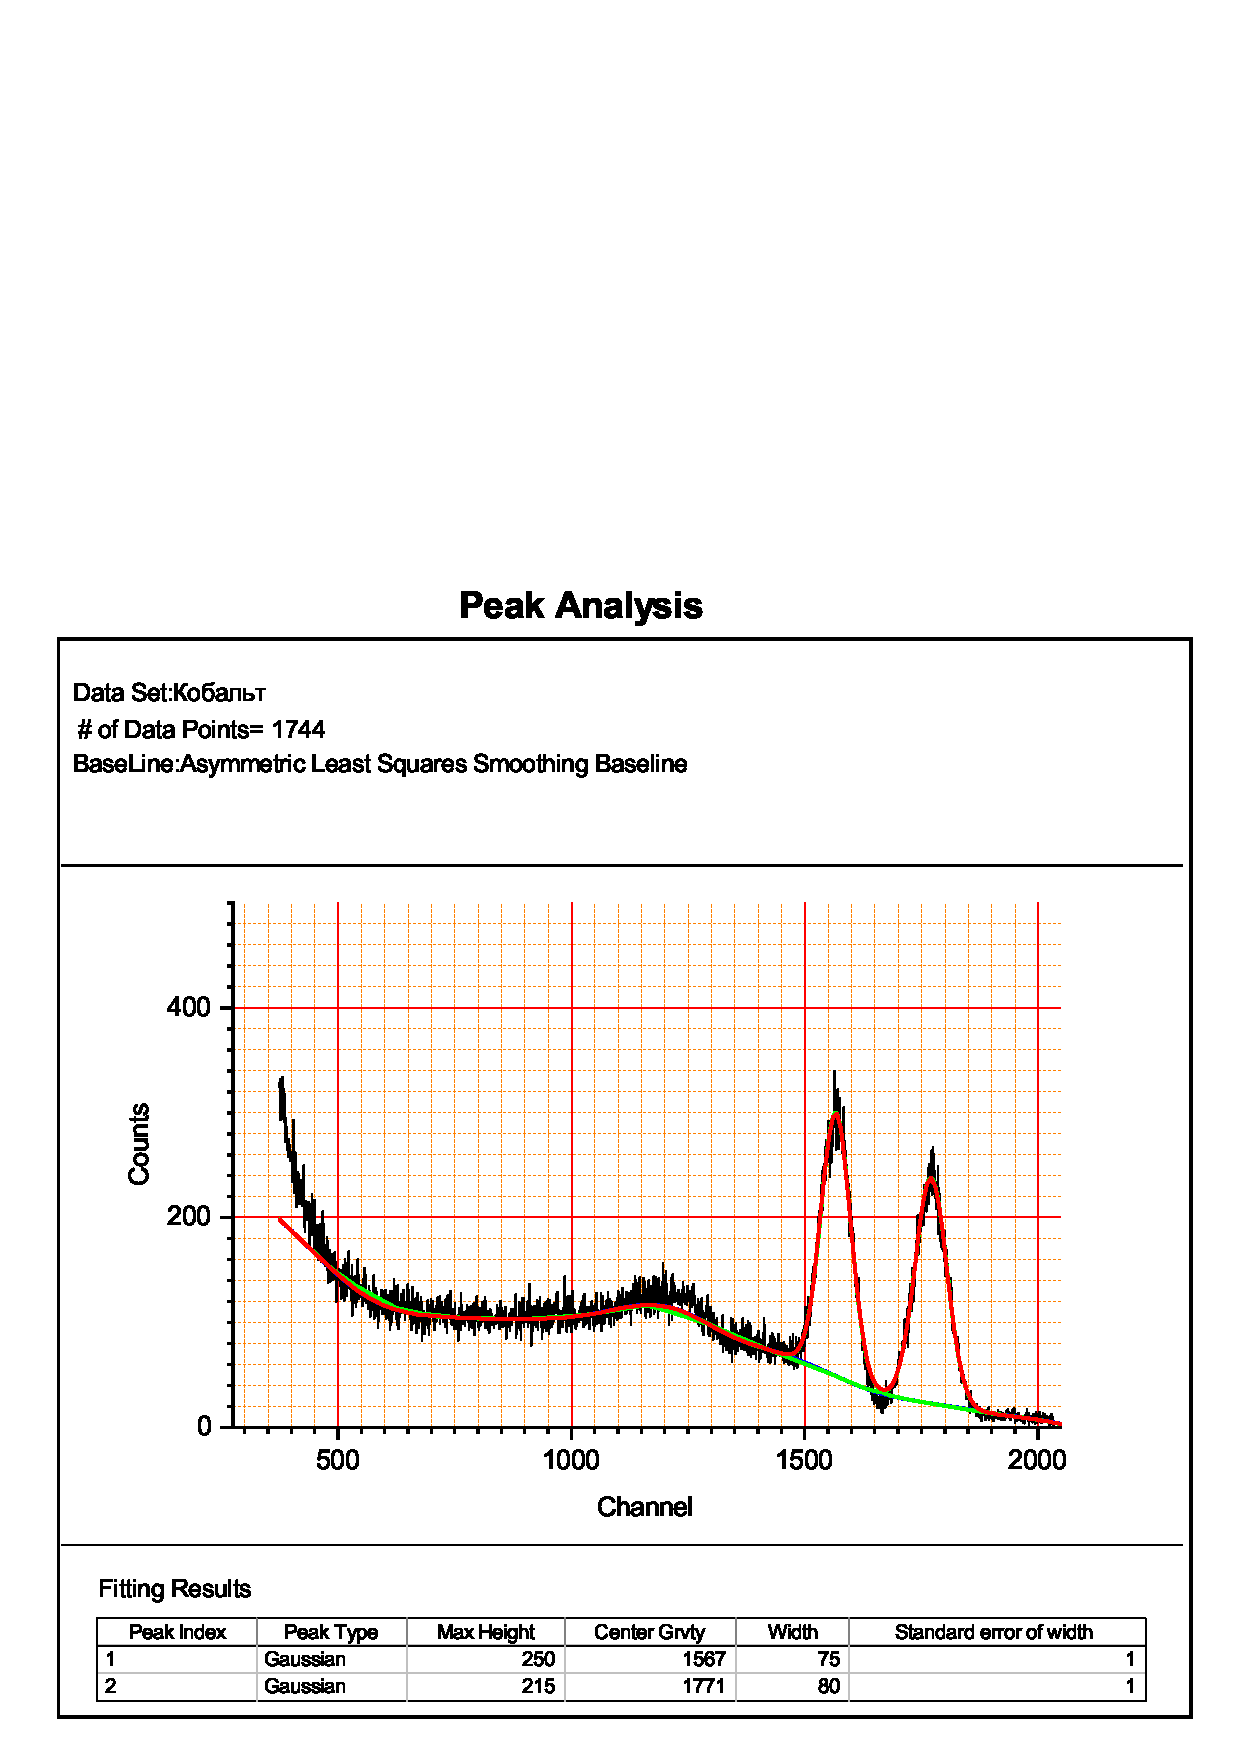
\includegraphics[width = 0.6\textwidth]{2.png}
\centering
\caption{Схема экспериментальной установки.}
\end{figure}


\section*{Выполнение и обработка данных}
Включив электронагреватель термостата, исследуем температурную зависимость ($p$--$n$)-перехода. Результаты измерений представлены в Таблице 1. Погрешность измерения сопротивления магазина взята $\sigma_{R_\text{м}} = 1~\text{Ом}$, напряжения на термопаре $\sigma_{V_{\text{терм}}} = 10~\text{мкВ}$. Темперутра считалась как 
\[T = \dfrac{V_{\text{терм}}[\text{мкВ}]}{41} + 25,~[^\circ \text{С}],\]
здесь $25~^\circ \text{С}$ -- температура сосуда Дюара, в которого помещён второй контакт термопары.


\begin{table}[h]
\begin{tabular}{|c|c|c|c|c|c|c|c|c|c|c|c|c|}
\hline
$R_\text{м}$, Ом       & 230  & 131  & 101  & 70   & 52   & 41   & 30   & 25   & 19   & 15   & 12   & 9    \\ \hline
$V_{\text{терм}}$, мкВ        & 0    & 210  & 400  & 600  & 800  & 1000 & 1200 & 1400 & 1600 & 1800 & 2000 & 2200 \\ \hline
$T$,$^{\circ}\text{C}$ & 25.0 & 30.1 & 34.8 & 39.6 & 44.5 & 49.4 & 54.3 & 59.1 & 64.0 & 68.9 & 73.8 & 78.7 \\ \hline
$R_g$, Ом              & 2300 & 1310 & 1010 & 700  & 520  & 410  & 300  & 250  & 190  & 150  & 120  & 90   \\ \hline
\end{tabular}
\centering
\caption{Результаты измерений.}
\end{table}
На основании этих данных построим график зависимости $\ln R_g$ от $1/T$, он представлен на Рис. 3
\begin{figure}[h]
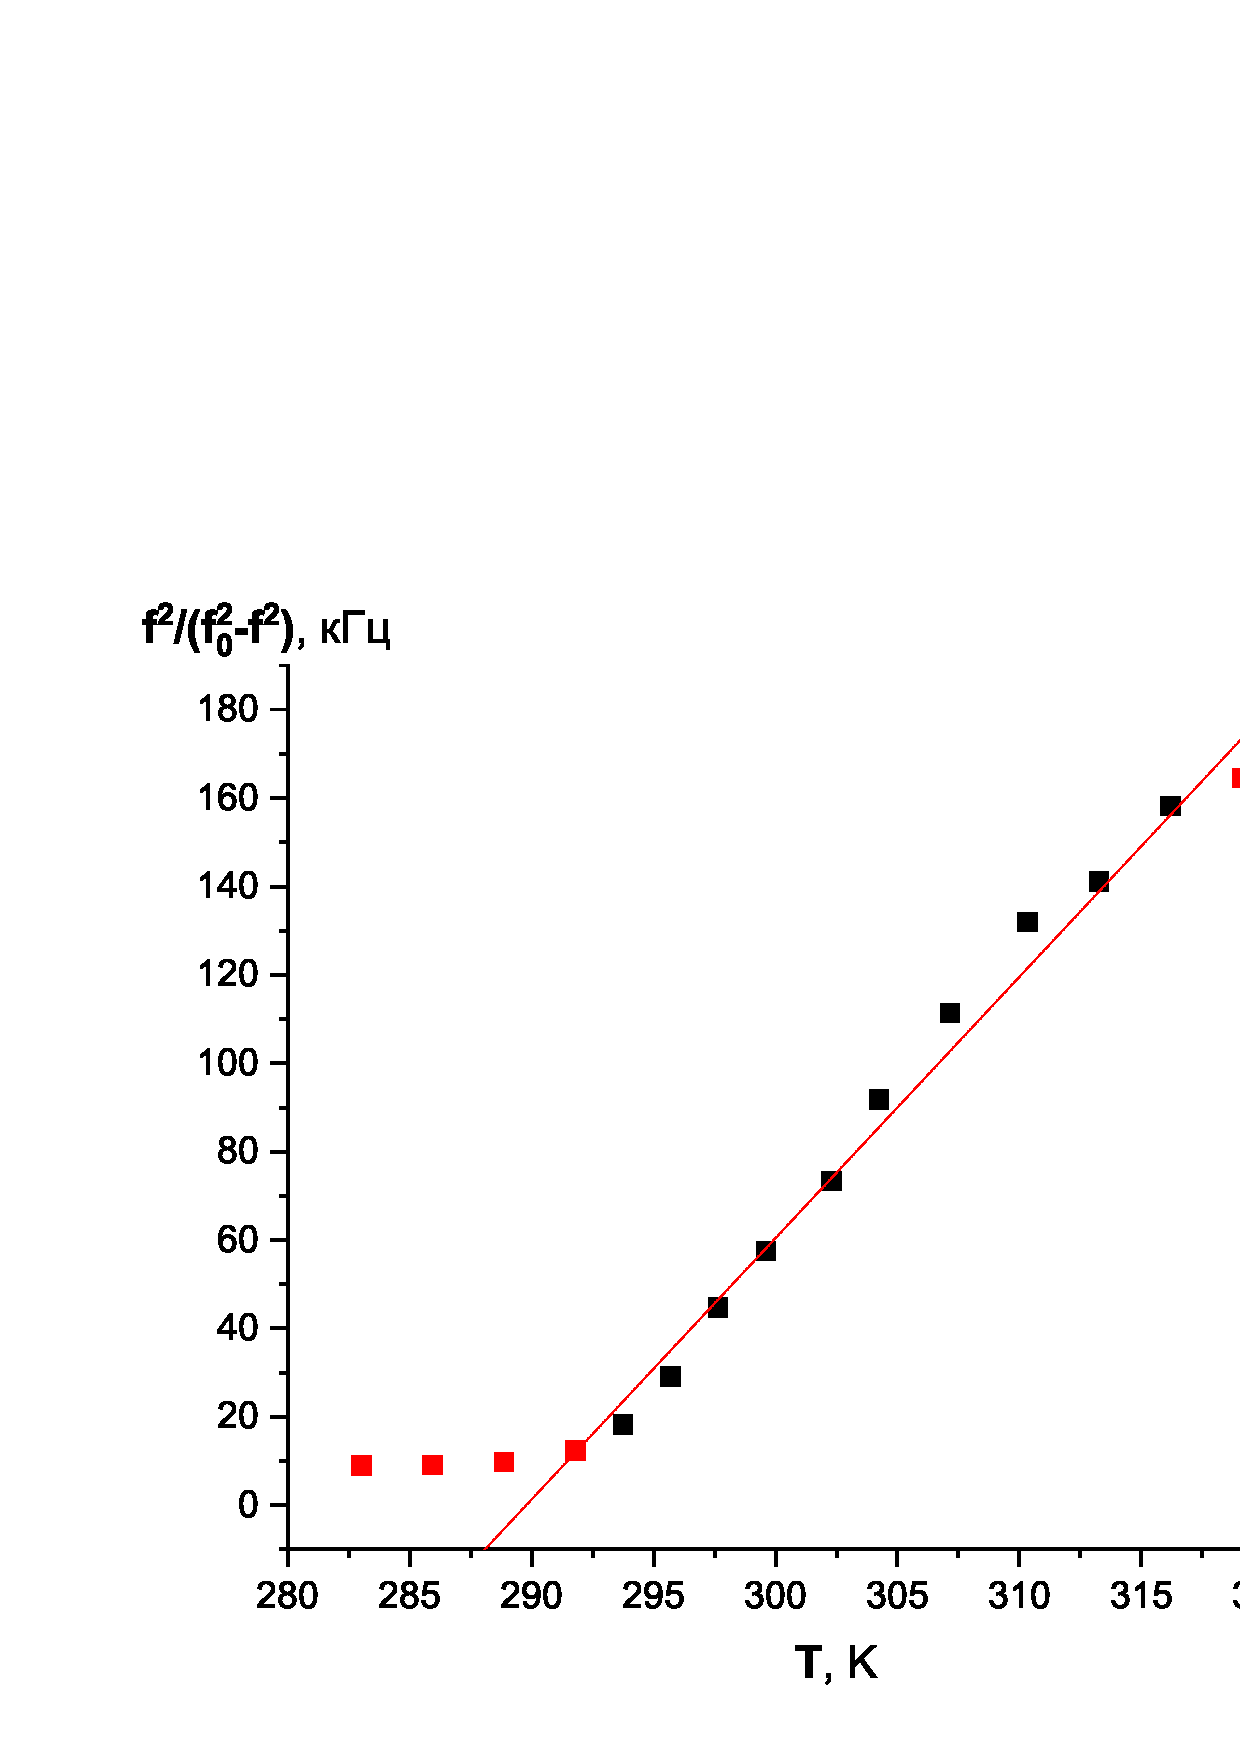
\includegraphics[width = 0.6\textwidth]{1.pdf}
\centering
\caption{Зависимость $\ln R_g$ от $1/T$.}
\end{figure}
Аппроксимируя зависимость прямой, получим 
\[\dfrac{d(\ln R)}{d(1/T)} = 6050 \pm 130~\text{К}^{-1}.\]
Тогда с учётом формулы (\ref{3}) разность потенциалов на переходе равна
\[\Delta V = 0.52 \pm 0.11~\text{В}.\]
\section*{Обсуждение}
В ходе работы было исследована температурная зависимость дифференциального сопротивления полупроводника, была определена контактная разность потенциалов ($p$--$n$)-перехода $\Delta V = 0.52 \pm 0.11~\text{В}$. В пособии \cite{laba} оценочно подсчитано значение $\Delta V = 0.35~\text{В}$, по порядку совподающие с полученным, но лежащее за пределами одного стандартного отклонения. Причиной может служить неточность определения уравновешенности моста по картине на экране осциллографа.

\begin{thebibliography}{9}
\bibitem{laba} 
Игошин Ф.Ф., Самарский Ю.А., Ципенюк Ю.М.
\textit{Лабораторный практикум по общей физики: Учеб. пособие для вузов. Т3. Квантовая физика.}. 
М.: Физматкнига - 2005.
\end{thebibliography}
\end{document}










